% Define the subtitle of the page
\title{Delving In}

% Begin the content of the page
\subsection{Delving In}

Edward enables black box inference for probability models. Its design reflects
the building blocks for inference and model checking. Here we describe the
motivation behind Edward's design and specify its internal workings.

Edward is named after the innovative statistician
\href{https://en.wikipedia.org/wiki/George_E._P._Box}{George Edward
Pelham Box}. Edward follows Box's philosophy of statistics and machine
learning.

First gather data from a real-world process. Then cycle through Box's
loop:

\begin{enumerate}
\item Build a probabilistic model of the process
\item Reason about the process given model and data
\item Criticize the model, revise and repeat
\end{enumerate}

\hspace*{100px}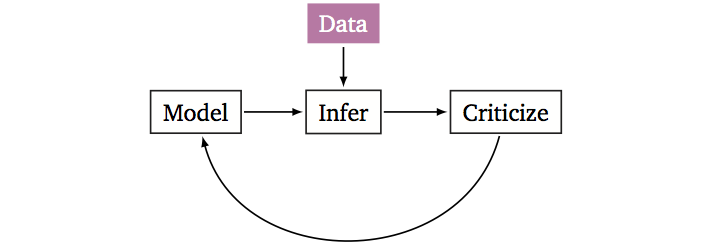
\includegraphics{images/model_infer_criticize.png}

Here's a toy example. A child flips a coin ten times, with the data of
outcomes being \texttt{{[}0,\ 1,\ 0,\ 0,\ 0,\ 0,\ 0,\ 0,\ 0,\ 1{]}}. We
are interested in the probability that the coin lands heads. First,
build a model: assume the coin flips are independent and land heads with
the same probability. Second, reason about the process: use an algorithm
to infer the model given data. Third, criticize the model: analyze
whether the model captures the real-world process of coin flips. If it
doesn't, then revise the model and repeat.

This process defines the design of Edward. Here are the four
primary objects that enable the above analysis. 

\subsubsection{Data}

\texttt{Data} objects are containers that contain measurements. The
structure of these objects must match the inputs of the probabilistic
model.

\begin{verbatim}
data = ed.Data(np.array([0, 1, 0, 0, 0, 0, 0, 0, 0, 1]))
\end{verbatim}

\paragraph{Models}\label{models}

There are two types of model objects in Edward:

\begin{enumerate}
\def\labelenumi{\arabic{enumi}.}
\tightlist
\item
  Probability models of data
\item
  Variational models of latent variables
\end{enumerate}

We can specify probability models of data using NumPy/SciPy, TensorFlow,
PyMC3, or Stan. Here is a model of coin flips using a
\href{https://en.wikipedia.org/wiki/Beta-binomial_distribution}{Beta-Bernoulli
distribution} in NumPy/Scipy.

\begin{verbatim}
class BetaBernoulli(PythonModel):
    """p(x, z) = Bernoulli(x | z) * Beta(z | 1, 1)
    """
    def _py_log_prob(self, xs, zs):
        n_samples = zs.shape[0]
        lp = np.zeros(n_samples, dtype=np.float32)
        for s in range(n_samples):
            lp[s] = beta.logpdf(zs[s, :], a=1.0, b=1.0)
            for n in range(len(xs)):
                lp[s] += bernoulli.logpmf(xs[n], p=zs[s, :])
        return lp
\end{verbatim}

This describes a Bayesian model, which is a joint distribution of data
and latent variables \texttt{z}. With this model and data of coin flips,
we aim to reason about \texttt{z}, the probability that the coin lands
heads. The posterior distribution of \texttt{z} captures our reasoning:
its mean describes our best guess of the probability, and its variance
describes our uncertainty around our best guess. In this toy model, we
know that the posterior is a Beta distribution. Let us assume we do not
know its parameters in closed form.

Edward can employ variational inference to infer this posterior, which
finds the closest distribution within a specified family. Initialize an
empty \texttt{Variational()} model. Then add a Beta distribution to the
variational model.

\begin{verbatim}
variational = Variational()
variational.add(Beta())
\end{verbatim}

With this syntax, we can build rich variational models to describe the
latent variables in our data models. (More documentation on this coming
soon.)

\paragraph{Inference}\label{inference}

\texttt{Inference} objects infer latent variables of models given data.
Edward currently supports a variety of variational inference algorithms.
These take as input a probability model, a variational model, and data.

Here we use mean-field variational inference.

\begin{verbatim}
inference = ed.MFVI(model, variational, data)
\end{verbatim}

(For the technical audience, the mean-field assumption of a fully
factorized approximation is moot here. We're dealing with a
one-dimensional latent variable.)

Calling \texttt{inference.run} runs the inference algorithm until
convergence. It recovers a Beta distribution with mean 0.25 and variance
0.12. 0.25 is our best guess of the probability that the coin lands
heads.

\paragraph{Criticism}\label{criticism}

{[}In Progress{]}




It also includes \textbf{features} such as
\begin{itemize}
\item \href{https://www.tensorflow.org}{TensorFlow} for backend computation,
  which includes automatic differentiation, GPU support, computational
  graphs, optimization, and TensorBoard
\item A library for probability distributions in TensorFlow
\item Documentation and tutorials
\item Examples demonstrating state-of-the-art generative models and
  inference
\end{itemize}


\subsubsection{A complete example: the Beta-Bernoulli
model}\label{a-complete-example-the-beta-bernoulli-model}

Here is a complete script, defining the data, model, and the variational
model. We run mean-field variational inference for \texttt{10000}
iterations at the end. The same example is also available in cases where
the model is written in
\href{https://github.com/blei-lab/edward/blob/master/examples/beta_bernoulli_stan.py}{Stan},
\href{https://github.com/blei-lab/edward/blob/master/examples/beta_bernoulli_pymc3.py}{PyMC3}
and
\href{https://github.com/blei-lab/edward/blob/master/examples/beta_bernoulli_tf.py}{TensorFlow}
respectively.

\begin{verbatim}
"""A simple coin flipping example. The model is written in NumPy/SciPy.

Probability model
    Prior: Beta
    Likelihood: Bernoulli
Variational model
    Likelihood: Mean-field Beta
"""
import edward as ed
import numpy as np

from edward.models import PythonModel, Variational, Beta
from scipy.stats import beta, bernoulli

class BetaBernoulli(PythonModel):
    """p(x, z) = Bernoulli(x | z) * Beta(z | 1, 1)
    """
    def _py_log_prob(self, xs, zs):
        # This example is pedagogical.
        # We recommend vectorizing operations in practice.
        n_minibatch = zs.shape[0]
        lp = np.zeros(n_minibatch, dtype=np.float32)
        for s in range(n_minibatch):
            lp[s] = beta.logpdf(zs[s, :], a=1.0, b=1.0)
            for n in range(len(xs)):
                lp[s] += bernoulli.logpmf(xs[n], p=zs[s, :])
        return lp

data = ed.Data(np.array([0, 1, 0, 0, 0, 0, 0, 0, 0, 1]))
model = BetaBernoulli()
variational = Variational()
variational.add(Beta())
inference = ed.MFVI(model, variational, data)

inference.run(n_iter=10000)
\end{verbatim}

\subsubsection{More Links}\label{more-links}

You can find more complicated examples in the
\href{https://github.com/blei-lab/edward/tree/master/examples}{\texttt{examples/}}
directory. We highlight several here:

\begin{itemize}
\tightlist
\item
  \href{https://github.com/blei-lab/edward/blob/master/examples/bayesian_linear_regression.py}{Bayesian
  linear regression}
\item
  \href{https://github.com/blei-lab/edward/blob/master/examples/hierarchical_logistic_regression.py}{Hierarchical
  logistic regression}
\item
  \href{https://github.com/blei-lab/edward/blob/master/examples/mixture_gaussian.py}{Mixture
  model of Gaussians}
\item
  \href{https://github.com/blei-lab/edward/blob/master/examples/gp_classification.py}{Gaussian
  process classification}
\item
  \href{https://github.com/blei-lab/edward/blob/master/examples/bayesian_nn.py}{Bayesian
  neural network}
\item
  \href{https://github.com/blei-lab/edward/blob/master/examples/mixture_density_network.py}{Mixture
  density network}
\item
  \href{https://github.com/blei-lab/edward/blob/master/examples/convolutional_vae.py}{Variational
  auto-encoder}
\end{itemize}

We think the library will make it significantly easier to do research in
machine learning and statistics. You can find more about this
\href{guide-research.md}{here}.

You can find more about Edward's design and philosophy, and how it
relates to other software \href{design.md}{here}.

\subsubsection{References}\label{references}

\begin{itemize}
\tightlist
\item
  David M Blei. Build, compute, critique, repeat: Data analysis with
  latent variable models. Annual Review of Statistics and Its
  Application, 1:203-232, 2014.
\end{itemize}
